\section{Ioniserende stråling}

\subsection{Innledning}

Det tredje eksperimentet handlet om ioniserende stråling og radioaktivitet. Hensikten med eksperimentet var å lære om hvordan observert strålingsmengde innen ett tidsintervall er påvirket av statistisk spredning, hvordan stråling blir absorbert, og bruk av Geiger-M$\ddot{\text{u}}$ller-teller. \medskip

Eksperimentet bygger på teori rundt stråling og radioaktivitet. I eksperimentet bruker vi $\gamma$-stråling med høy energi, en form for ioniserende elektromagnetisk stråling. Denne strålingen oppstår som et produkt av noen typer radioaktiv henfall, som er slik vi vil danne denne strålingen.

For en radioaktiv kjerne, vil det være en konstant sannsynlighet for desintegrasjon. En kjerne er enten desintegrert, eller ikke, som betyr at desintegrasjonen følger en Bernoulli-prosess, og fordi sannsynligheten for at kjernen desintegrerer er liten (for mange isotoper) kan vi finne sannsynligheten for et X antall desintegrasjoner over tiden $\Delta$t ved hjelp av en Poissonfordeling.

For dette eksperimentet vil vi bruke en Geiger-M$\ddot{\text{u}}$ller-teller, et instrument som måler antall ioniserte partikler. GM-telleren har et GM-rør, som plukker opp den ioniserende strålingen. 
Noe av denne strålingen (ca 1\%) vil treffe veggen på innsiden av røret og slå løs elektroner via fotoelektrisk effekt. Disse elektronene ioniserer gass-molekylene som befinner seg innad i GM-telleren, og GM-telleren kan måle dette. På denne måten kan vi få et mål på hvor intens en stråling er.\medskip

Formålet med eksperimentet var å måle og analysere dempning av ioniserende stråling gjennom en
absorbator med varierende tykkelse. Vi brukte bly som absorbator, og GM-telleren til å måle dempningen.

\subsection{Material og Metoder}

Til eksperimentet trengte vi Geiger-M$\ddot{\text{u}}$ller-teller (se fig \ref{GM}), radioaktiv kilde , en stoppeklokke (vi brukte mobiltelefon), en mobiltelefon som kan ta opp slow-motion video, skyvelære, og 6 blyplater.\medskip

\bigskip \hfil
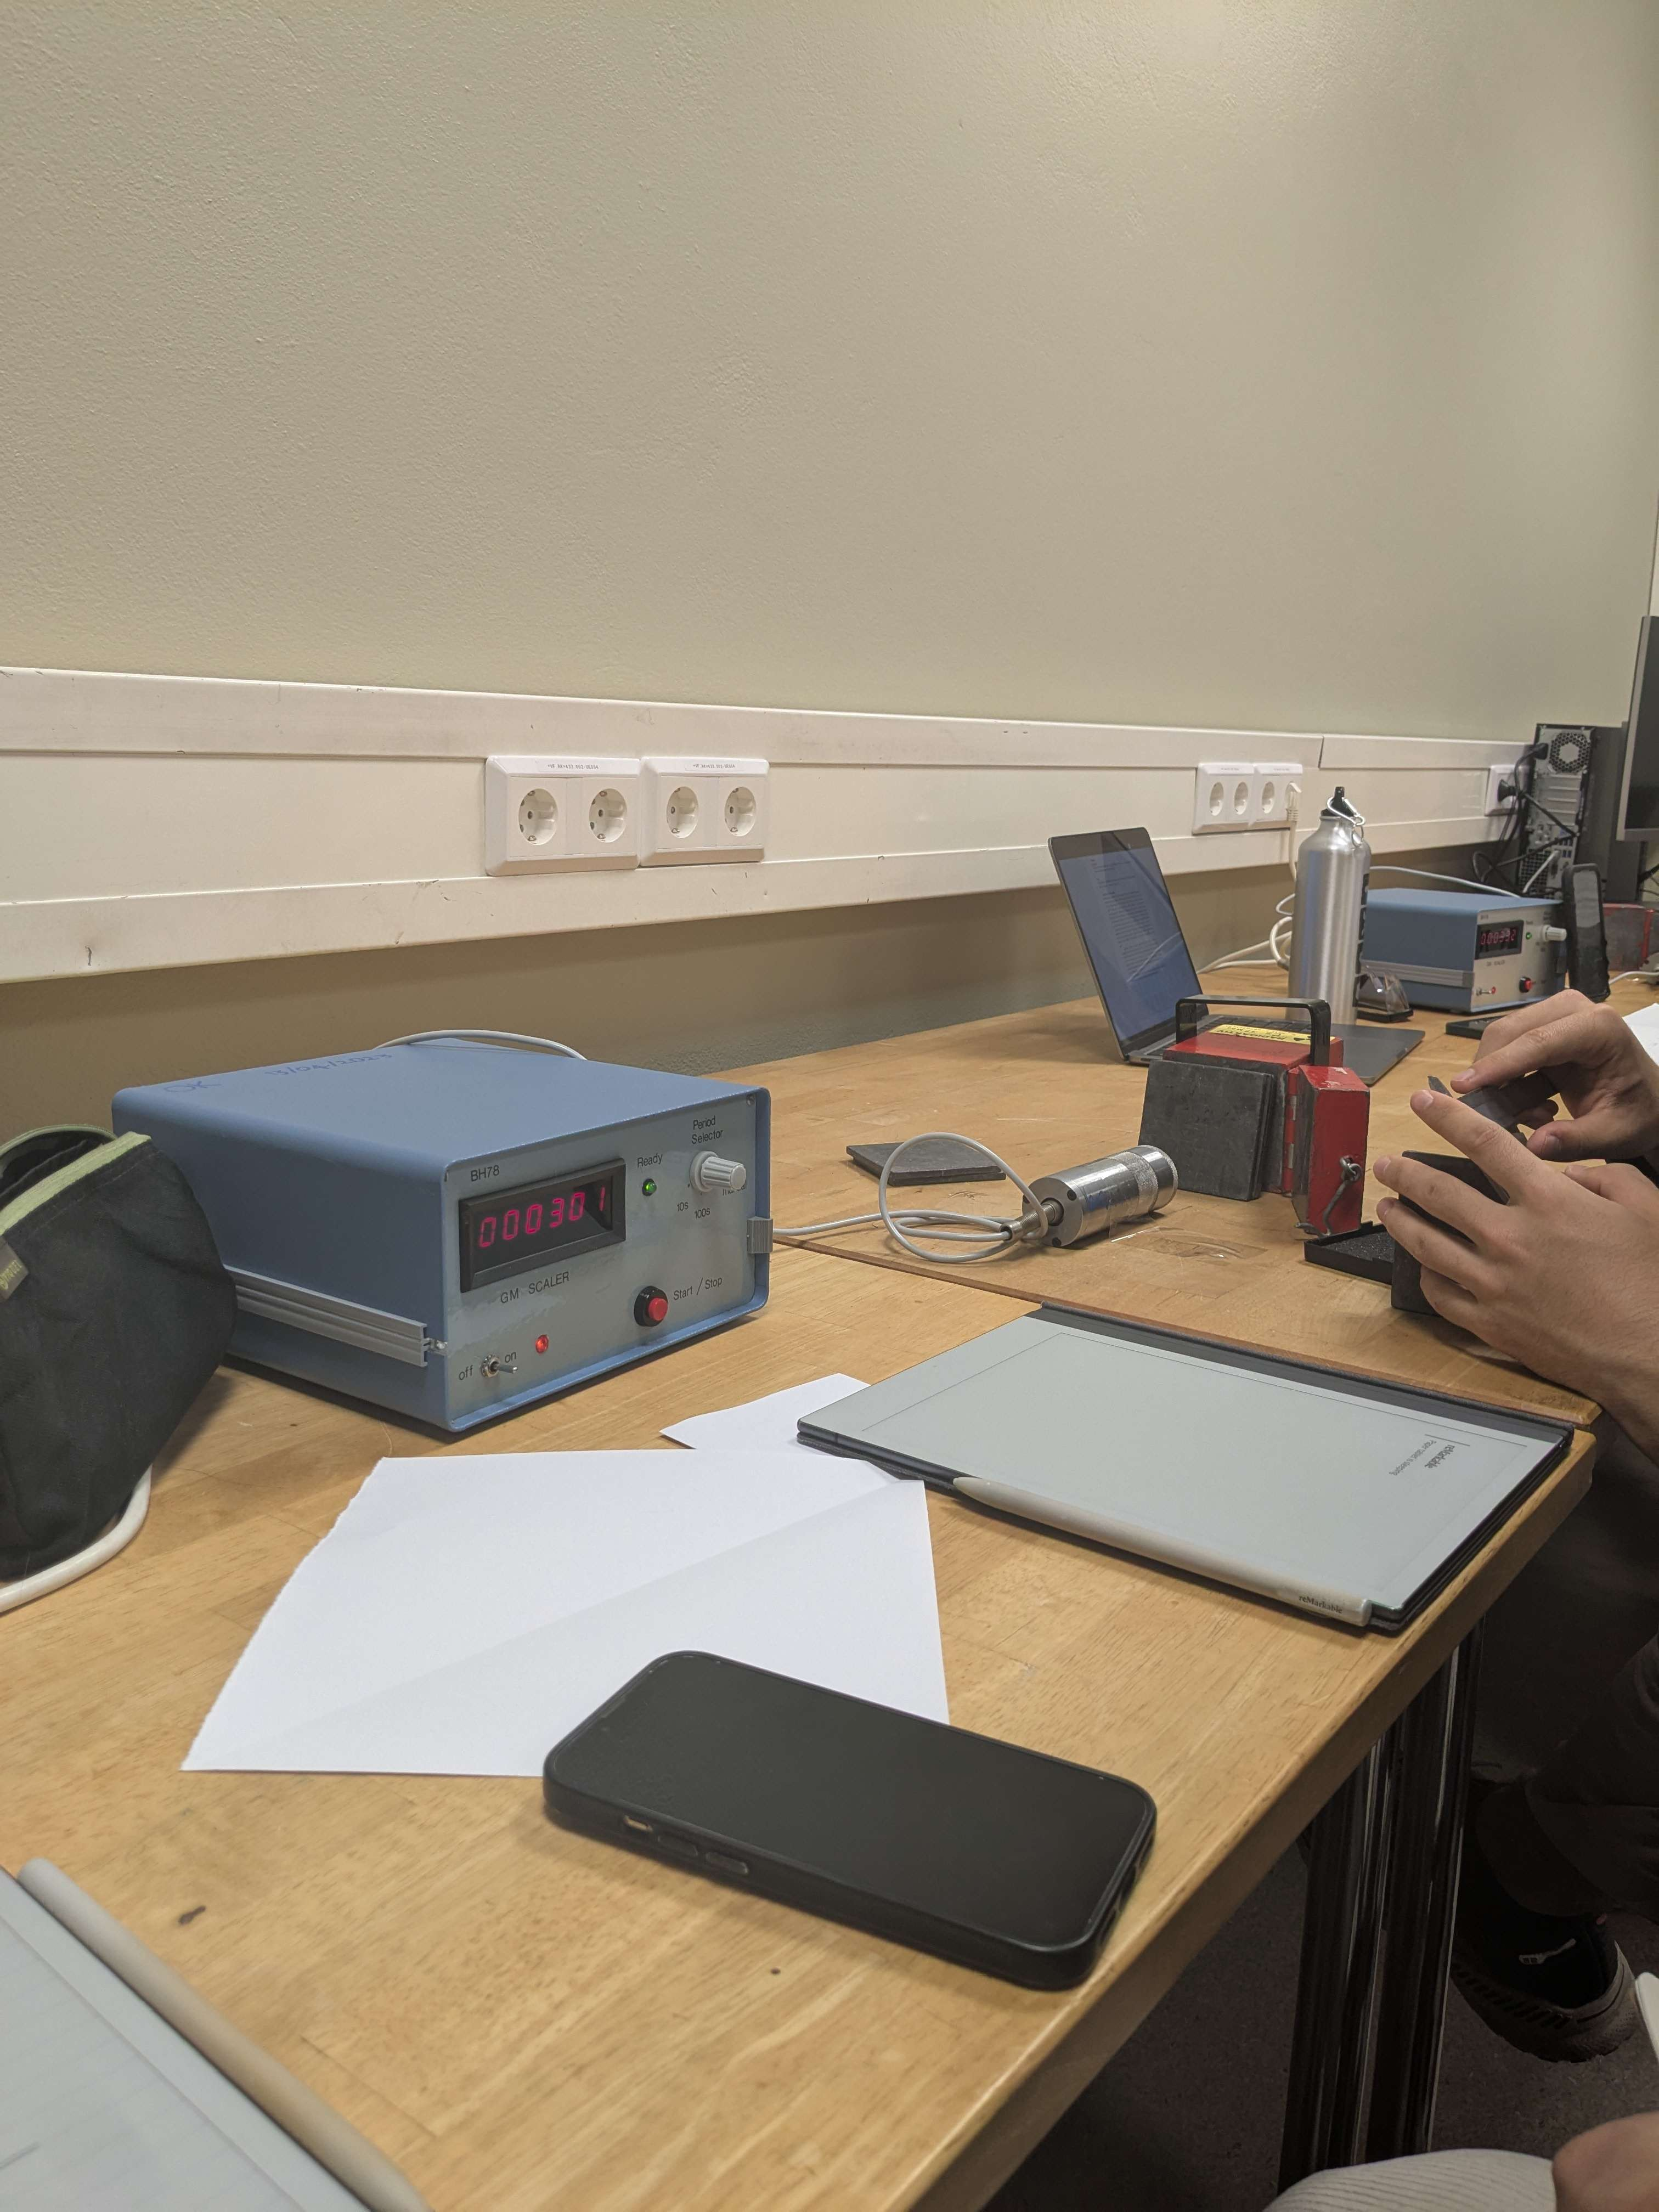
\includegraphics[scale = 0.05]{Figurer/GM-Counter.jpg} 
\captionof{figure}{Geiger-M$\ddot{\text{u}}$ller-telleren (blå), sammen med radioaktiv kilde (rødt), pekende mot GM-rør.}\label{GM}
\par \bigskip

Vi begynte med å måle bakgrunnstrålingen $I_b$. Vi plasserte alle 6 blyplatene foran GM-røret, skrudde på telleren uten noen radioaktiv kilde, og lot den stå på i 10 minutter. Så estimerte vi usikkerheten til $I_b$ ved å bruke at strålingen er Poisson-fordelt. Dette gir oss

\begin{align}
    u_{I_b} = \sqrt{I_b}  \label{u_b}
\end{align}

Vi brukte dette som bakgrunnsstrålingen fremover. \medskip

Så plasserte vi den radioaktive kilden vår foran GM-røret, og sørget for at det ikke bevegde seg under eksperimentet. Vi tok så 5 mål av hvor lang tid det tok for GM-telleren å samle 1000 tellinger, og fant snittet av disse målene. Etter dette, målte vi antall tellinger over snittiden for 1 - 6 blyplater. Før vi målte antall tellinger, målte vi tykkelsen på blyplaten vi la til. Siden tiden $\overline{t}$ var kort, plasserte vi stoppeklokken vår (mobiltelefon) ved siden av GM-telleren, og filmet telleren og klokken i slow-motion, slik at vi kunne plukke ut tiden mer nøyaktig.\medskip

For å finne usikkerheten i en sum av andre usikre variabler, brukte vi følgende formel
\begin{align}
    u_f = \sqrt{u_x^2 +u_y^2}\label{au2}
\end{align}

Mer generelt anvendte vi 

\begin{align}
    u_f^2 = \left(\frac{\delta f}{\delta x} u_x\right)^2 + \left(\frac{\delta f}{\delta y} u_y\right)^2\label{gu3}
\end{align}

Vi fant også relative usikkerheter ved følgende formel:
\begin{align}
    r_x = \frac{u_x}{\sqrt{x}}
\end{align}


Til slutt, plottet vi Strålingen mot blytykkelsen i python. Vi plottet også Strålingen log-transformert, slik at den ble lineær med blytykkelsen. For å gjøre dette, brukte vi følgende sammenheng:

\begin{align}
    I = I_0e^{-\mu_\gamma x} \implies \ln{I} = -\mu_\gamma x + \ln{I_0}\label{stbt}
\end{align}

Der $I_0$ er strålingen uten noen blyplater, og $\mu_\gamma$ er dempningskoeffisienten. 

\subsection{Resultater}

Bakgrunnstrålingen $I_b$ i løpet av 10 minutter ble målt til 266. Formel \ref{ub} gir oss da $u_{I_b} = \sqrt{266} = 16,31$. Dette bruker vi som bakgrunnsstrålingen fremover. \medskip

Våre fem mål for tiden GM-telleren brukte på å samle 1000-tellinger uten noen blyplater, samt snittet av disse, ble som følger:

\begin{center}
\begin{tabular}{ | c | }
    \hline
    t\\ 
    \hline
    14.05\\ 
    \hline
    14.28\\ 
    \hline
    14.76\\ 
    \hline
    14.56\\ 
    \hline
    15.46\\ 
    \hline
\end{tabular}\;\;\;
\begin{tabular}{ | c | }
    \hline
    $\overline{t}$\\ 
    \hline
    14.622\\ 
    \hline
\end{tabular}
\captionof{table}{Målte tider for 1000 tellinger uten blyplater, sammen med snittet av disse tidene (i sekunder).}
\end{center}

Tykkelsen på de 6 blyplatene:

\begin{center}
\begin{tabular}{ | c | c | }
    \hline
    & dx\\ 
    \hline
    1 & 0.53\\ 
    \hline
    2 & 0.32\\ 
    \hline
    3 & 0.525\\ 
    \hline
    4 & 0.52\\ 
    \hline
    5 & 0.51\\ 
    \hline
    6 & 0.511\\ 
    \hline
\end{tabular}
\captionof{table}{Tykkelsen på de 6 blyplatene (i cm)}
\end{center}

Den samlede tabellen med alle mål tatt av GM-telleren:

\begin{center}
\begin{tabular}{ | c | c | c | c | c | }
    \hline
    Antall blyplater & Total Blytykkelse dx (cm) & $u_{dx}$ (cm) & Antall Målinger & standardavvik\\ 
    \hline
    1 & 0.53 & 0.0071 & 604 & 24.58\\ 
    \hline
    2 & 0.83 & 0.01 &381 & 19.52\\ 
    \hline
    3 & 1.38 & 0.012 &269 & 16.40\\ 
    \hline
    4 & 1.90 & 0.014 &130 & 11.40\\ 
    \hline
    5 & 2.40 & 0.016 &86 & 9.27\\ 
    \hline
    6 & 2.92 & 0.017 &42 & 6.48\\ 
    \hline
\end{tabular}
\captionof{table}{Antall blyplater, Totale blytykkelser, usikkerhet i disse blytykkelsene, antall målinger fra GM-telleren, og standardavvikene for disse målene.} \label{bigtable}
\end{center}

standardavvikene her er funnet fra formel \ref{u_b}, og usikkerhetene er funnet fra skyvelærens skalausikkerhet $u_{skala} = 0.05$ mm, skyvelærens avlesningsusikkerhet $u_{avles} = 0.05$ mm, og formel \ref{au2}.

Relative Usikkerheter for Blytykkelse og Antall målinger:

\begin{center}
\begin{tabular}{ | c | c | c |}
    \hline
    N plater & $r_x$ &  $r_n$\\ 
    \hline
    1 & 0.009753 & 1.0001\\ 
    \hline
    2 & 0.01097 & 1.0000\\ 
    \hline
    3 & 0.01021 & 0.9999\\ 
    \hline
    4 & 0.01015 & 0.9998\\ 
    \hline
    5 & 0.01032 & 0.9996\\ 
    \hline
    6 & 0.009948 & 0.9998\\  
    \hline
\end{tabular}
\captionof{table}{Relative usikkerheter for blytykkelse og antall målinger} 
\end{center}

Vi fikk følgende plott for Stråling mot blytykkelse:

\begin{center}
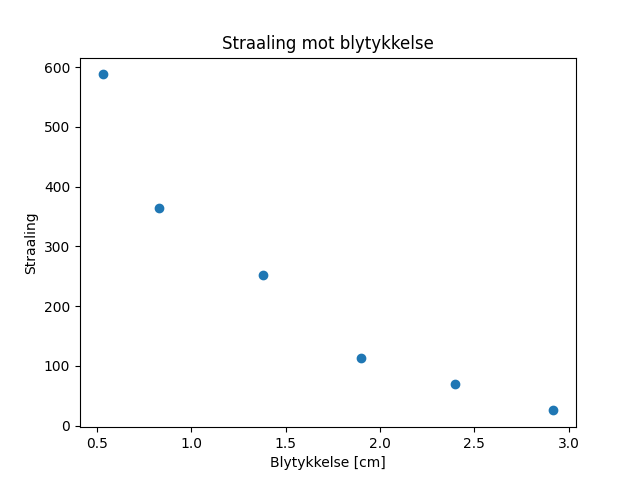
\includegraphics[scale=0.7]{Figurer/Straaling_Bly.png}
\end{center}

Så for log-transformerte data (ved bruk av formel \ref{stbt}):

\begin{center}
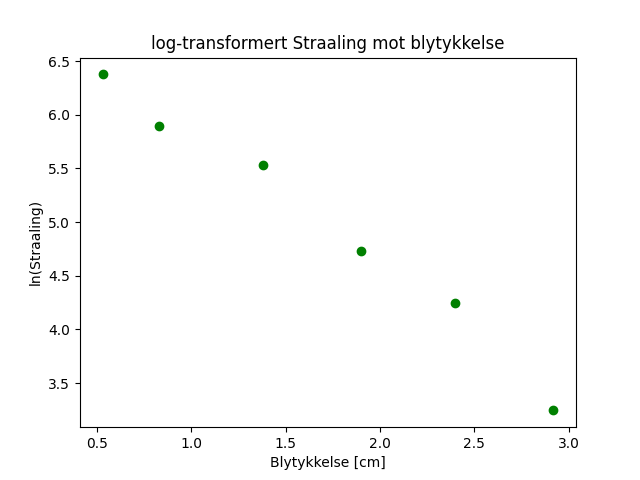
\includegraphics[scale=0.7]{Figurer/LogStraaling_Bly.png}
\end{center}

Vi tilpasset en lineær regresjonsmodell til dette plottet:

\begin{center}
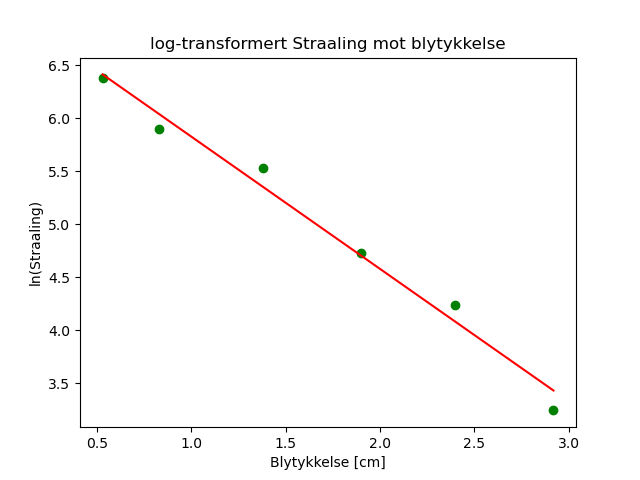
\includegraphics[scale=0.7]{Figurer/LogStraaling_Regresjon.png}
\end{center}

Denne regresjonsmodellen ga oss et uttrykk for  $\ln{I}$, og usikkerhetene i $\beta_0$ og $\beta_1$. Sammen med formelog $u_{\n{I}}$:

\begin{align*}
    (\ln{(I)})(x) &= -1.247014\cdot x + 7.075217\\
    u_{\n{I}} &= \sqrt{(x\cdot 0.082)^2 + 0.153^2}
\end{align*}

Programmet ga oss også et estimat for blytykkelsen nødvendig for at 90\% og 99\% av strålingen skal absorberes:

\begin{center}
\begin{tabular}{ | c | c | c | }
    \hline
    Prosentandel & 90\% & 99\%\\ 
    \hline
    Blytykkelse & 5.107 & 5.617\\ 
    \hline
    Usikkerhet & 0.4458 & 0.48534\\ 
    \hline
\end{tabular}
\captionof{table}{Nødvendig blytykkelse (i cm) for å absorbere 90\% og 99\% av strålingen.}
\end{center}

[Usikkerhet for dette!!!]

\subsection{Diskusjon}

Selv om det ikke ble spesifisert i oppgaven, valgte vi å ta flere mål av tiden GM-telleren brukte på å samle 1000 tellinger, og når vi da bruker snitt-tiden, får vi et noe mer nøyaktig mål (ideelt sett skulle vi hatt flere målinger av t).\medskip

Målene våre for blyplatenes tykkelser er ganske nøyaktige, grunnet skyvælærens lave usikkerheter. Når vi ser på en sammenheng som dette, der både tykkelsene og tellingene er usikre, kan vi se i tabell \ref{bigtable} at dersom vi bruker tellingenes standardavvik som usikkerheter, at disse er mye større enn usikkerhetene for for tykkelsen i platene. Samtidig øker usikkerheten i tykkelsene med antall plater, mens usikkerheten i tellingene minker, så om den totale blytykkelsen blir stor, kan dette forholdet endres.\medskip

[Noe om relativ usikkerhet???]\medskip

I det første plottet, der stråling plottes direkte mot blytykkelse, ser vi punkter som danner en kurve som blir mindre bratt når blytykkelsen øker. Dette samsvarer med formel \ref{stbt}, hvor vi kan se at I er omvendt proporsjonal med $e^x$, som danner en graf som ser slik ut.

I det andre plottet, der $\ln{I}$ plottes mot blytykkelsen, får vi punkter som danner en rett linje. Dette samsvarer igjen med formel \ref{stbt}, der vi kan se at $\ln{I}$ er lineær med x. Sammen med utrykket vi fikk fra regresjonen, kan vi også da finne at $\mu_\gamma$ er stigningen i dette utrykket, 1.247014. Samtidig er ikke denne modellen helt perfekt. Det lineære utrykket gir oss at $\ln{I_0} = 7.075217$, som gir oss $I_0 = e^{7.075217} = 1096.6$, som ikke er helt nøyaktig. Dette kunne bli løst med flere blyplater, som kunne gitt oss en bedre modell. Vi kunne også fått en bedre modell ved å måle tellinger for flere kombinasjoner av platene, i stedet for å kun måle i rekkefølge.\medskip

[Noe om å lære å bruke GM-teller??]
